\documentclass[12pt]{article}
\usepackage[final]{graphicx}
\usepackage{amsmath}
\usepackage{minted}
\usepackage{multicol}
\usepackage{subcaption}
\usepackage{tabularx}
\usepackage[english]{babel}

\title{Transformer open circuit \& short circuit test}
\author{}
\date{}

\begin{document}
\vspace*{\fill}
\begin{center}

    \emph{Heaven's Light is Our Guide} \\
    \textbf{Rajshahi Universiy of Engineering and Technology} \\

    \begin{figure}[h]
        \centering
        
\includegraphics[scale=.34]{images/RUET_logo.png}
        \label{fig:ruet_logo}
    \end{figure}
    \vspace{5mm}

    \textbf{Course Code}\\
    ECE 2208\\
    \vspace{3mm}
    \textbf{Course Title}\\
    Electrical Machines - I Sessional

    \vspace{5mm}
    \textbf{Experiment Date:} {October 4, 2023,}\\
    \textbf{Submission Date:} {October 18, 2023}\\

    \vspace{5mm}
    \textbf{Lab Report 1:} Polarity test of a transformer.\\

    \vspace{15mm}

    \begin{tabular}{c|c}
        \textbf{Submitted to} & \textbf{Submitted by} \\
        Md. Omaer Faruq Goni  & Md. Tajim An Noor     \\
        Lecturer              & Roll: 2010025         \\
        Dept of ECE, RUET     &                       \\
    \end{tabular}

\end{center}
\vspace*{\fill}

\pagebreak

\tableofcontents

\maketitle
\section{Introduction}
These two tests, open \& short circuit test are done on a transformer to
\begin{itemize}
    \item Calculate core and copper losses of transformer.
    \item The equivalent circuit of transformer.
    \item Voltage regulation of transformer.
    \item Efficiency of transformer.
\end{itemize}
\subsection{Open Circuit Test}

These two tests are also economical as they're done without loading the transformer.\\\\
Open circuit test or no load test is performed to determine 'no load loss (Core loss)' and 'no load current I\textsubscript{0}'.\\\\
In this test usually the high voltage (HV) winding is kept open and the low voltage (LV) winding is connected to supply. A wattmeter (W), ammeter (A) and voltmeter (V) are connected to the LV winding as shown in the figure. Then , applied voltage is slowly increased from zero to rated value of the LV side with the help of a variac.Readings are taken after the supply reaches the rated voltage.\\\\
The ammeter reading gives the no load current I\textsubscript{0}. As I\textsubscript{0} itself is very small, the voltage drops due to this current can be neglected.\\\\
The input power is indicated by the wattmeter (W). And as the other side (HV) of transformer is open circuited, there is no output power. Hence, this input power only consists of core losses and copper losses. As described above, no-load current is so small that these copper losses can be neglected. Hence, now the input power is almost equal to the total core losses. Thus, the wattmeter reading gives the core losses of the transformer.\\\cite{openShort}

\subsection{Short Circuit Test}
The LV side of transformer is short circuited and wattmeter (W), voltmeter (V) and ammeter (A) are connected on the HV side of the transformer. Voltage is applied to the HV side and increased from the zero until the \emph{ammeter} reading equals the rated current. All the readings are taken at this rated current.\\\\
The ammeter reading gives primary equivalent of full load current (I\textsubscript{sc}).\\\\
The voltage applied for full load current is very small as compared to rated voltage. Hence, core loss due to small applied voltage can be neglected. Thus, the wattmeter reading can be taken as copper loss in the transformer.\cite{openShort}

\subsection{Circuit Diagrams}
\begin{figure}[htbp!]
    \centering
    % 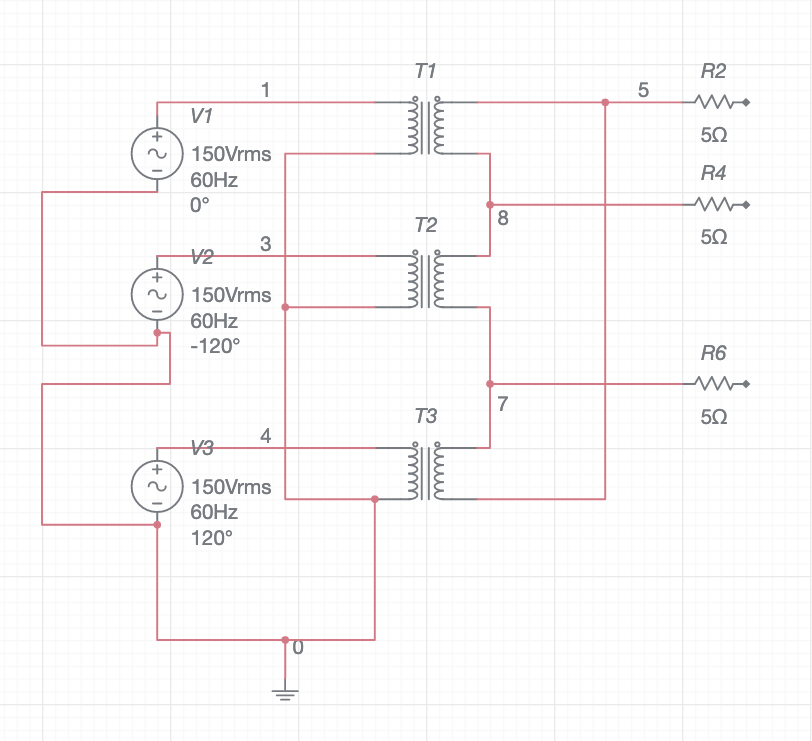
\includegraphics[width=.8\linewidth]{images/output/ydel.png}
    \caption{Circuit diagrams for Y-$\Delta$ three transformer connection.}
    \label{fig:fig}
\end{figure}
\vspace{\fill}

\pagebreak
\section{Tools Used}
\begin{itemize}
    \item Transformer (150V - 1A)
    \item Connecting wires
    \item Ammeter (0A - 5A)
    \item Voltmeter (0V - 120V)
    \item Wattmeter
    \item AC supply (220V)
    \item Variac (0-250V)
\end{itemize}

\section{Data \& Calculation}
\subsection{Data Table:}
\begin{table}[H]
    \centering
    \caption{Open Circuit Test}
    \begin{tabular}{|c|c|c|c|}
        \hline
        Test               & \bf{Input Voltage (V)} & \bf{Current (A)} & \bf{Power (W, Loss)} \\
        \hline
        \bf{Open Circuit}  & 150                    & 0.18             & 12.5                 \\
        \hline
        \bf{Short Circuit} & 14                     & 1                & 11.25                \\
        \hline
    \end{tabular}
\end{table}

\subsection{Calculation:}
Loss Calculation:\\
\[\text{Total loss} = \text{Copper Loss} + \text{Core Loss}\]
\[= 12.5+11.25 = 23.75\]\\
Calculating efficiency:
\begin{align*}
    \text{Efficiency} & = |\frac{\text{Input Power - Losses}}{\text{Input}} |\times100\% \\
                      & = |\frac{\text{V*I - Losses}}{\text{Input}} |\times100\%         \\
                      & = |\frac{14\times1 - (23.75)}{14\times 1}|\times 100\%           \\
                      & = 69.64\%
\end{align*}

\subsection{Result}

Core Loss   = \(12.5 W\)   \\
Copper Loss  = \(11.25 W\) \\
Total Loss = \(23.75 W\)\\
Efficiency = \(69.64\%\)

\section{Discussion}
From the experiment, it can be seen that copper loss of a transformer depends on current, and iron loss depends on voltage. Thus, total transformer loss depends on volt-ampere (VA).\cite{openShort}

\section{Conclusion}
Since this experiment was done with AC supply, utmost caution was exercised to avoid any accident.
\bibliographystyle{IEEEtran}
\bibliography{ref}

\end{document}